\documentclass[11pt, a4paper]{article}
\usepackage{graphicx}
\usepackage[a4paper, top=2.2cm, bottom=2.2cm, left=2cm, right=2cm]{geometry}
\usepackage[english]{babel}
\usepackage[T1]{fontenc}
\usepackage[utf8]{inputenc}
\usepackage{lmodern}
\usepackage{booktabs}
\usepackage{array}
\usepackage{enumitem}
\usepackage{titlesec}
\titlespacing*{\section}{0pt}{1.2\baselineskip}{0.8\baselineskip}
\titlespacing*{\subsection}{0pt}{1.0\baselineskip}{0.5\baselineskip}
\titlespacing*{\subsubsection}{0pt}{1.0\baselineskip}{0.5\baselineskip}
\usepackage[hidelinks]{hyperref}
\usepackage{textcomp}
\usepackage{framed}

\title{Design Report: Distributed Prime Finding Platform}
\author{AFS-Like Distributed File System}
\date{}

\begin{document}

\maketitle
\thispagestyle{empty}
\pagestyle{headings}

\section{Executive Summary}

This report presents the design and implementation of a fault-tolerant distributed system for finding prime numbers in large datasets. The system has two components: an AFS-like distributed file system and a distributed prime-finding application.

The file system uses a replicated leader-follower architecture employing the Raft consensus algorithm. The application uses a coordinator-worker model to distribute computation, with workers processing data chunks in parallel.

Fault tolerance is achieved through active-passive replication for the coordinator, Raft consensus for file servers, and consistent global snapshots for crash recovery and task resumption.

\begin{description}
    \item[System Scale:] Multiple Workers, Replicated Coordinators, and Replicated File Servers.
    \item[Communication:] gRPC protocol
    \item[Key Algorithms:] Global snapshots, Raft consensus, exponential backoff with failover
\end{description}

\section{System Model}

The system finds unique prime numbers and stores them in a distributed file server. It comprises three process types communicating via gRPC over an asynchronous network with possible crash-fail errors.

\begin{description}
    \item[\textbf{File Servers (Replicated):}] A Raft-based replicated cluster for high-availability storage.
    \item[\textbf{Application Coordinator (Replicated):}] A central replicated service managing task assignment and snapshots.
    \item[\textbf{Application Workers:}] A pool of processes performing computation and interacting with File Servers.
\end{description}

\section{System Assumptions and Limitations}

\subsection{Assumptions}
\begin{description}
    \item[Network:] Eventual connectivity with transient partitions. Crash-fail model with 30–60 s gRPC timeouts.
    \item[Storage:] Durable POSIX-compliant storage; no silent disk corruption.
    \item[Processes:] Fail-stop failures, independent and uncorrelated.
\end{description}

\subsection{Limitations}
\begin{description}
    \item[Byzantine Failures:] Not supported.
    \item[Extreme Delays:] Treated as process failures.
    \item[Concurrent Failures:] Manual intervention required for coordinator or quorum loss.
\end{description}

\section{Part 1: AFS-Like Distributed File System}

The file system provides highly available, read-optimized storage for datasets and results.

\subsection{Architecture and Core RPCs}

The design implements an AFS-like whole-file caching model. Clients fetch the full file on open and perform local reads. Writes are flushed on close.

\begin{itemize}
    \item \texttt{UploadFile(stream FileChunk)}: worker uploads
    \item \texttt{FetchFile(FetchRequest)}: worker downloads
    \item \texttt{RequestVote(VoteRequest)}: Raft leader election
    \item \texttt{Heartbeat(HeartbeatRequest)}: Raft authority maintenance
    \item \texttt{ReplicateFile(stream Req)}: leader data replication to followers
\end{itemize}


\begin{figure}[htbp]
    \centering
    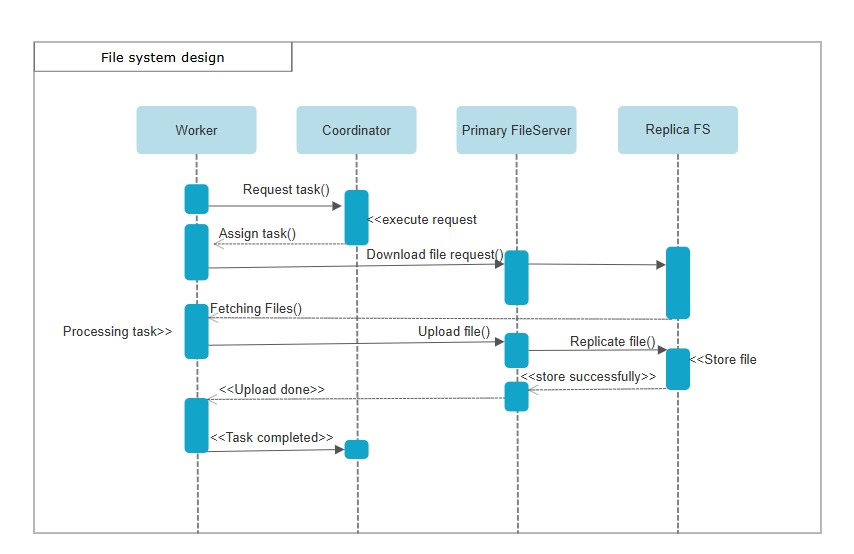
\includegraphics[width=0.9\textwidth]{system-design.jpeg}
    \caption{File system design sequence diagram.}
    \label{fig:system_design}
\end{figure}


\subsection{File Server Fault Tolerance (Raft)}

\begin{itemize}
    \item \textbf{Leader Election:} Servers start as Followers. If no heartbeats are received within a randomized timeout, a server becomes Candidate, requests votes, and if it wins a majority, becomes Leader.
    \item \textbf{Write Path:} Only the Leader handles \texttt{UploadFile}, commits data locally, and replicates via \texttt{ReplicateFile}.
    \item \textbf{Read Path:} Any server can serve reads, enabling load balancing.
\end{itemize}

\pagebreak

\section{Part 2: Distributed Prime Finding Application}

The application layer manages distributed computation via a Coordinator-Worker model.

\subsection{Application Fault Tolerance}

\begin{itemize}
    \item \textbf{Coordinator Failure:} A backup runs in active-passive mode. On primary failure, workers reconnect to the backup.
    \item \textbf{Worker Failure:} Workers send heartbeats to the Coordinator. Missing heartbeats mark the worker dead and trigger task reassignment.
    \item \textbf{Task Re-assignment:} Failed tasks are reassigned. Workers save progress to the file system as snapshots, enabling resumed computation.
\end{itemize}

\section{Failure Handling Summary}

\begin{table}[htbp]
    \centering
    \caption{Failure Types and Recovery Mechanisms}
    \label{tab:failures}
    \begin{tabular}{@{}p{3.5cm}p{4cm}p{5cm}p{3cm}@{}}
        \toprule
        \textbf{Failure Type} & \textbf{Detection} & \textbf{Recovery}               & \textbf{Guarantee}       \\ \midrule
        Client/Worker Crash   & Alive lock file    & Snapshot reload and task resume & Eventually consistent    \\
        Coordinator Crash     & gRPC timeout       & Failover to secondary           & High availability        \\
        FileServer Crash      & gRPC timeout       & Raft leader election            & Linearizable consistency \\
        Network Partition     & Deadline exceeded  & Exponential backoff and retry   & Eventually consistent    \\
        Data Corruption       & Checksum mismatch  & Reject and retry                & Strong integrity         \\
        Task Failure          & Heartbeat timeout  & Task reassignment               & At-least-once semantics  \\ \bottomrule
    \end{tabular}
\end{table}

\end{document}
